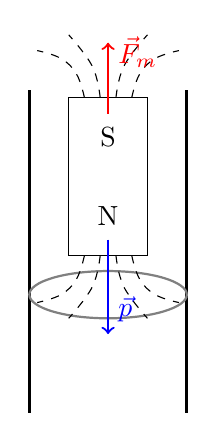
\begin{tikzpicture}

\draw [very thick] (-0.5,-0.5) -- (-0.5,3.6);
\draw [very thick]  (1.5,-0.5) -- (1.5,3.6);
\draw [thick, gray] (0.5,1) ellipse (1 and 0.3);
\draw  (0,3.5) rectangle (1,1.5);
\node at (0.5,2) {N};
\node at (0.5,3) {S};
\draw [dashed] plot[smooth, tension=.7] coordinates {(0.2,1.5) (0.1,1.2) (-0.1,1) (-0.4,0.9)};
\draw [dashed] plot[smooth, tension=.7] coordinates {(0.4,1.5) (0.3,1.1) (0,0.7)};
\draw  [dashed]plot[smooth, tension=.7] coordinates {(0.6,1.5) (0.7,1.1) (1,0.7)};
\draw [dashed] plot[smooth, tension=.7] coordinates {(0.8,1.5) (0.9,1.2) (1.1,1) (1.4,0.9)};
\draw [dashed] plot[smooth, tension=.7] coordinates {(0.2,3.5) (0.1,3.8) (-0.1,4) (-0.4,4.1)};
\draw[dashed]  plot[smooth, tension=.7] coordinates {(0.8,3.5) (0.9,3.8) (1.1,4) (1.4,4.1)};
\draw [dashed] plot[smooth, tension=.7] coordinates {(0.6,3.5) (0.7,3.9) (1,4.3)};
\draw[dashed]  plot[smooth, tension=.7] coordinates {(0.4,3.5) (0.3,3.9) (0,4.3)};
\draw [->, thick, blue](0.5,1.7) -- (0.5,0.5)node [midway, below right]{$\vec{p}$};
\draw  [->, thick, red] (0.5,3.3) -- (0.5,4.2)node [midway, above right]{$\vec{F}_m$};
\end{tikzpicture}